\documentclass{standalone}
\usepackage{tikz}
\usetikzlibrary{patterns, positioning}
\usepackage[sfdefault]{ClearSans} %% option 'sfdefault' activates Clear Sans as the default text font
\usepackage[T1]{fontenc}

\begin{document}
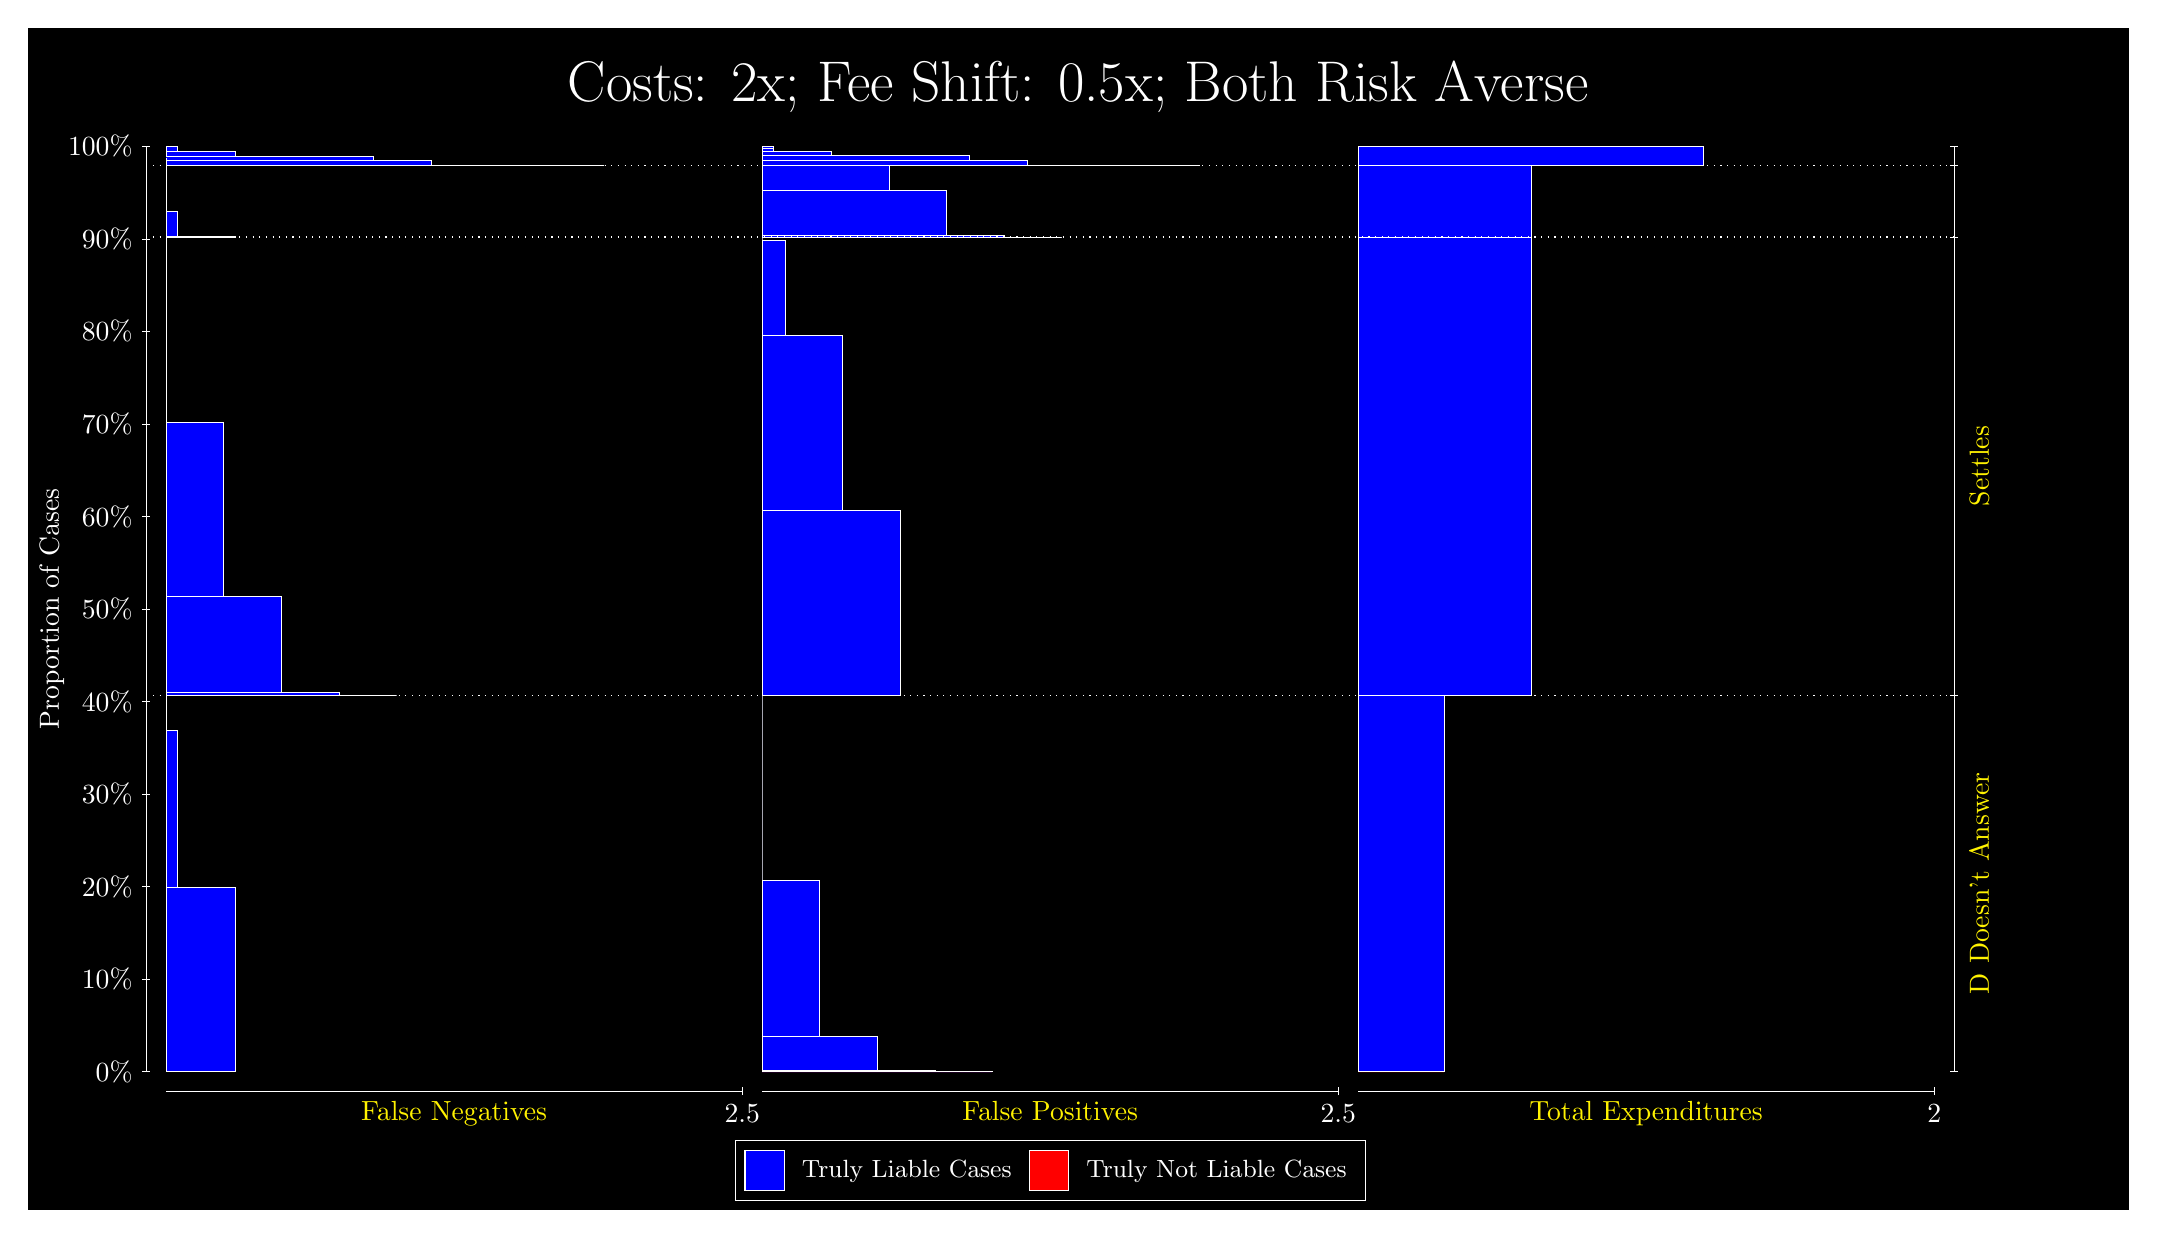
\begin{tikzpicture}
\draw[fill=black] (0,0) rectangle (26.667,15);
\draw[text=white] (0,13.5) rectangle (26.667,15) node[midway] {\huge Costs: 2x; Fee Shift: 0.5x; Both Risk Averse};
\draw[white, very thin] (1.5,1.75) -- (1.5,13.5);
\node[rotate=90, text=white, anchor=center] at (0.3, 7.625) {Proportion of Cases};
\draw[white, very thin] (1.45,1.75) -- (1.55,1.75);
\node[text=white, anchor=east] at (1.45, 1.75) {0\%};
\draw[white, very thin] (1.45,2.925) -- (1.55,2.925);
\node[text=white, anchor=east] at (1.45, 2.925) {10\%};
\draw[white, very thin] (1.45,4.1) -- (1.55,4.1);
\node[text=white, anchor=east] at (1.45, 4.1) {20\%};
\draw[white, very thin] (1.45,5.275) -- (1.55,5.275);
\node[text=white, anchor=east] at (1.45, 5.275) {30\%};
\draw[white, very thin] (1.45,6.45) -- (1.55,6.45);
\node[text=white, anchor=east] at (1.45, 6.45) {40\%};
\draw[white, very thin] (1.45,7.625) -- (1.55,7.625);
\node[text=white, anchor=east] at (1.45, 7.625) {50\%};
\draw[white, very thin] (1.45,8.8) -- (1.55,8.8);
\node[text=white, anchor=east] at (1.45, 8.8) {60\%};
\draw[white, very thin] (1.45,9.975) -- (1.55,9.975);
\node[text=white, anchor=east] at (1.45, 9.975) {70\%};
\draw[white, very thin] (1.45,11.15) -- (1.55,11.15);
\node[text=white, anchor=east] at (1.45, 11.15) {80\%};
\draw[white, very thin] (1.45,12.325) -- (1.55,12.325);
\node[text=white, anchor=east] at (1.45, 12.325) {90\%};
\draw[white, very thin] (1.45,13.5) -- (1.55,13.5);
\node[text=white, anchor=east] at (1.45, 13.5) {100\%};

\draw[white, very thin] (24.457,1.75) -- (24.457,13.5);
\draw[white, very thin] (24.407,1.75) -- (24.507,1.75);
\node[anchor=west] at (24.407, 1.75) {};
\draw[white, very thin] (24.407,6.5291) -- (24.507,6.5291);
\node[anchor=west] at (24.407, 6.5291) {};
\draw[white, very thin] (24.407,12.349) -- (24.507,12.349);
\node[anchor=west] at (24.407, 12.349) {};
\draw[white, very thin] (24.407,13.26) -- (24.507,13.26);
\node[anchor=west] at (24.407, 13.26) {};
\draw[white, very thin] (24.407,13.5) -- (24.507,13.5);
\node[anchor=west] at (24.407, 13.5) {};

\draw[white, very thin, fill=blue] (1.75,1.75) rectangle (2.6283,4.0963);
\draw[white, very thin, fill=blue] (1.75,4.0963) rectangle (1.8964,6.0856);
\draw[white, very thin, fill=red] (1.75,6.0856) rectangle (1.75,6.0856);
\draw[white, very thin, fill=blue] (1.75,6.0856) rectangle (1.75,6.5291);
\draw[white, very thin, fill=blue] (1.75,6.5291) rectangle (4.6775,6.5291);
\draw[white, very thin, fill=blue] (1.75,6.5291) rectangle (3.9457,6.5689);
\draw[white, very thin, fill=blue] (1.75,6.5689) rectangle (3.2138,7.7821);
\draw[white, very thin, fill=blue] (1.75,7.7821) rectangle (2.4819,9.9999);
\draw[white, very thin, fill=red] (1.75,9.9999) rectangle (1.75,9.9999);
\draw[white, very thin, fill=blue] (1.75,9.9999) rectangle (1.75,12.349);
\draw[white, very thin, fill=blue] (1.75,12.349) rectangle (2.6283,12.352);
\draw[white, very thin, fill=blue] (1.75,12.352) rectangle (1.8964,12.67);
\draw[white, very thin, fill=red] (1.75,12.67) rectangle (1.75,12.67);
\draw[white, very thin, fill=blue] (1.75,12.67) rectangle (1.75,13.26);
\draw[white, very thin, fill=blue] (1.75,13.26) rectangle (7.3123,13.26);
\draw[white, very thin, fill=blue] (1.75,13.26) rectangle (6.5805,13.26);
\draw[white, very thin, fill=blue] (1.75,13.26) rectangle (5.8486,13.263);
\draw[white, very thin, fill=blue] (1.75,13.263) rectangle (5.1167,13.318);
\draw[white, very thin, fill=blue] (1.75,13.318) rectangle (4.3848,13.369);
\draw[white, very thin, fill=blue] (1.75,13.369) rectangle (4.092,13.369);
\draw[white, very thin, fill=blue] (1.75,13.369) rectangle (3.6529,13.369);
\draw[white, very thin, fill=blue] (1.75,13.369) rectangle (3.3602,13.37);
\draw[white, very thin, fill=blue] (1.75,13.37) rectangle (2.6283,13.37);
\draw[white, very thin, fill=blue] (1.75,13.37) rectangle (2.6283,13.439);
\draw[white, very thin, fill=blue] (1.75,13.439) rectangle (1.8964,13.44);
\draw[white, very thin, fill=blue] (1.75,13.44) rectangle (1.8964,13.495);
\draw[white, very thin, fill=red] (1.75,13.495) rectangle (1.75,13.495);
\draw[white, very thin, fill=blue] (1.75,13.495) rectangle (1.75,13.5);
\draw[white, very thin, fill=red] (9.3189,1.75) rectangle (12.246,1.75);
\draw[white, very thin, fill=blue] (9.3189,1.75) rectangle (12.246,1.7501);
\draw[white, very thin, fill=blue] (9.3189,1.7501) rectangle (11.515,1.7659);
\draw[white, very thin, fill=blue] (9.3189,1.7659) rectangle (10.783,2.1935);
\draw[white, very thin, fill=blue] (9.3189,2.1935) rectangle (10.051,4.1828);
\draw[white, very thin, fill=blue] (9.3189,4.1828) rectangle (9.3189,6.5291);
\draw[white, very thin, fill=red] (9.3189,6.5291) rectangle (11.075,6.5291);
\draw[white, very thin, fill=blue] (9.3189,6.5291) rectangle (11.075,8.8778);
\draw[white, very thin, fill=blue] (9.3189,8.8778) rectangle (10.344,11.096);
\draw[white, very thin, fill=blue] (9.3189,11.096) rectangle (9.6116,12.309);
\draw[white, very thin, fill=blue] (9.3189,12.309) rectangle (9.3189,12.349);
\draw[white, very thin, fill=red] (9.3189,12.349) rectangle (13.125,12.349);
\draw[white, very thin, fill=blue] (9.3189,12.349) rectangle (13.125,12.349);
\draw[white, very thin, fill=blue] (9.3189,12.349) rectangle (12.393,12.366);
\draw[white, very thin, fill=blue] (9.3189,12.366) rectangle (11.661,12.938);
\draw[white, very thin, fill=blue] (9.3189,12.938) rectangle (10.929,13.256);
\draw[white, very thin, fill=blue] (9.3189,13.256) rectangle (10.197,13.26);
\draw[white, very thin, fill=red] (9.3189,13.26) rectangle (14.881,13.26);
\draw[white, very thin, fill=blue] (9.3189,13.26) rectangle (14.881,13.26);
\draw[white, very thin, fill=red] (9.3189,13.26) rectangle (14.149,13.26);
\draw[white, very thin, fill=blue] (9.3189,13.26) rectangle (14.149,13.26);
\draw[white, very thin, fill=red] (9.3189,13.26) rectangle (13.417,13.26);
\draw[white, very thin, fill=blue] (9.3189,13.26) rectangle (13.417,13.265);
\draw[white, very thin, fill=blue] (9.3189,13.265) rectangle (12.686,13.321);
\draw[white, very thin, fill=blue] (9.3189,13.321) rectangle (11.954,13.39);
\draw[white, very thin, fill=blue] (9.3189,13.39) rectangle (11.222,13.391);
\draw[white, very thin, fill=red] (9.3189,13.391) rectangle (10.929,13.391);
\draw[white, very thin, fill=blue] (9.3189,13.391) rectangle (10.929,13.391);
\draw[white, very thin, fill=blue] (9.3189,13.391) rectangle (10.49,13.391);
\draw[white, very thin, fill=blue] (9.3189,13.391) rectangle (10.197,13.441);
\draw[white, very thin, fill=red] (9.3189,13.441) rectangle (10.197,13.441);
\draw[white, very thin, fill=blue] (9.3189,13.441) rectangle (10.197,13.442);
\draw[white, very thin, fill=blue] (9.3189,13.442) rectangle (9.4652,13.474);
\draw[white, very thin, fill=blue] (9.3189,13.474) rectangle (9.4652,13.497);
\draw[white, very thin, fill=blue] (9.3189,13.497) rectangle (9.3189,13.5);
\draw[white, very thin, fill=red] (16.888,1.75) rectangle (17.986,1.75);
\draw[white, very thin, fill=blue] (16.888,1.75) rectangle (17.986,6.5291);
\draw[white, very thin, fill=red] (16.888,6.5291) rectangle (19.083,6.5291);
\draw[white, very thin, fill=blue] (16.888,6.5291) rectangle (19.083,12.349);
\draw[white, very thin, fill=red] (16.888,12.349) rectangle (19.083,12.349);
\draw[white, very thin, fill=blue] (16.888,12.349) rectangle (19.083,13.26);
\draw[white, very thin, fill=red] (16.888,13.26) rectangle (21.279,13.26);
\draw[white, very thin, fill=blue] (16.888,13.26) rectangle (21.279,13.5);
\draw[white, dotted] (1.5,6.5291) -- (24.457,6.5291);
\draw[white, dotted] (1.5,12.349) -- (24.457,12.349);
\draw[white, dotted] (1.5,13.26) -- (24.457,13.26);
\draw[white, very thin] (1.75,1.5) -- (9.0689,1.5);
\node[text=yellow, anchor=north] at (5.4094, 1.5) {False Negatives};
\draw[white, very thin] (9.0689,1.45) -- (9.0689,1.55);
\node[text=white, anchor=north] at (9.0689, 1.45) {2.5};

\draw[white, very thin] (9.3189,1.5) -- (16.638,1.5);
\node[text=yellow, anchor=north] at (12.978, 1.5) {False Positives};
\draw[white, very thin] (16.638,1.45) -- (16.638,1.55);
\node[text=white, anchor=north] at (16.638, 1.45) {2.5};

\draw[white, very thin] (16.888,1.5) -- (24.207,1.5);
\node[text=yellow, anchor=north] at (20.547, 1.5) {Total Expenditures};
\draw[white, very thin] (24.207,1.45) -- (24.207,1.55);
\node[text=white, anchor=north] at (24.207, 1.45) {2};

\node[text=yellow, centered, rotate=90] at (24.777, 4.1396) {D Doesn't Answer};
\node[text=yellow, centered, rotate=90] at (24.777, 9.4388) {Settles};



\draw (12.978300999999998,1.5) node[draw=none] (baseCoordinate) {};
\begin{scope}[align=center]
        \matrix[scale=0.5, draw=white, below=0.5cm of baseCoordinate, nodes={draw}, column sep=0.1cm]{
            \node[rectangle, draw, minimum width=0.5cm, minimum height=0.5cm, fill=blue] {}; &
            \node[draw=none, font=\small, text=white] (B) {Truly Liable Cases}; &
            \node[rectangle, draw, minimum width=0.5cm, minimum height=0.5cm, fill=red] {}; &
            \node[draw=none, font=\small, text=white] (B) {Truly Not Liable Cases}; \\
            };
\end{scope}

\end{tikzpicture}
\end{document}